%
%\color{blue}

\subsection{Glyph: \glyph{Phenotype}}
\label{sec:phenotype}

A biochemical network can generate phenotypes or affect biological
processes.  Such processes can take place at different levels and are
independent of the biochemical network itself.  To represent these
processes in a map, \SBGNERLone defines the \glyph{phenotype} glyph.

\begin{glyphDescription}

\glyphSboTerm SBO:0000358 ! phenotype
\glyphOrigin Non-applicable
\glyphTarget Non-applicable
\glyphEndPoint A \glyph{phenotype} is represented by an elongated
hexagon, as illustrated in \fig{phenotype}. It is identified by a label placed in an
unbordered box containing a string of characters.  The characters can be
distributed on several lines to improve readability, although this is not
mandatory.  The label box must be attached to the center of the
\glyph{phenotype} container.  The label may spill outside of the container.

\end{glyphDescription}
 
\begin{figure}[H]
  \centering
  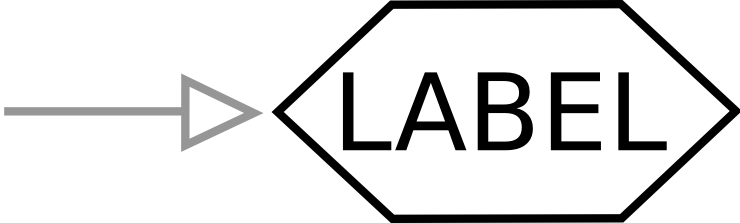
\includegraphics[scale = 0.3]{images/phenotype}
  \caption{The \ER glyph for \glyph{phenotype}.}
  \label{fig:phenotype}
\end{figure}

\begin{figure}[H]
  \centering
  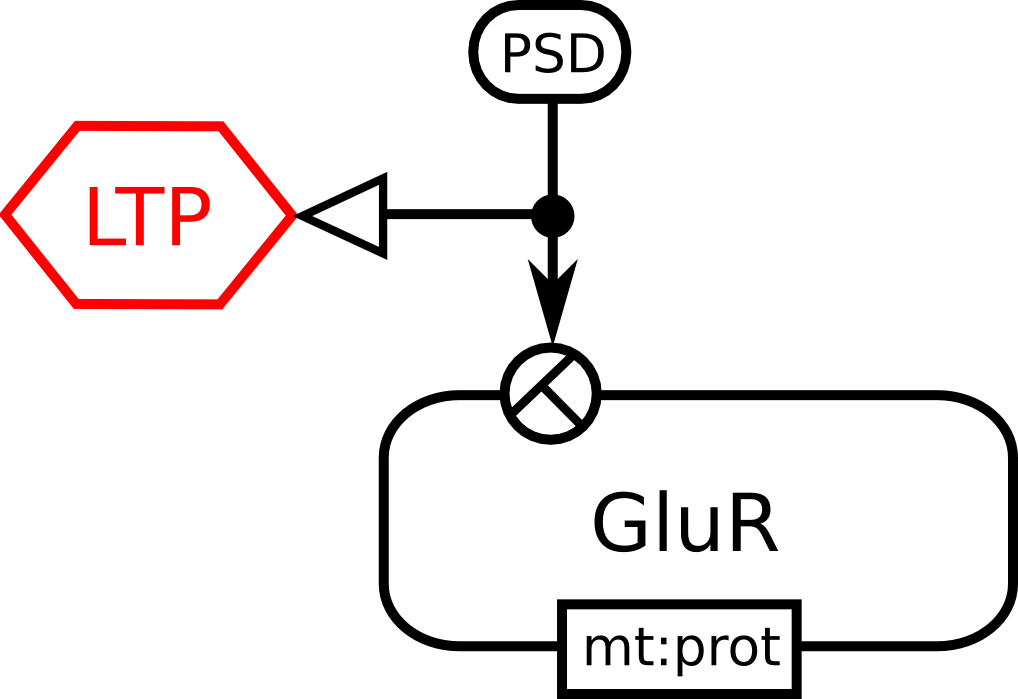
\includegraphics[scale = 0.5]{examples/ex-phenotype}
  \caption{Example of a \glyph{phenotype} ``Long Term Potentiation (LTP)'' enhanced when the entity ``GluR'' is present in the post-synaptic density.}
  \label{fig:ex-phenotype}
\end{figure}

%\normalcolor
